\section{Durchführung}
\label{sec:Durchführung}
Der experimentelle Aufbau ist in dem Röntgengerät integriert (siehe Abb. \ref{fig:aufbau}).
Zum wesentlichen Bestandteil des Aufbaus gehört die Kupfer-Röntgenröhre, der Plexiglas-Streuer/LiF-Kristall und das Geiger-Müller-Zählrohr.
Das Röntgengerät kann entweder über einen Computer gesteuert oder manuell bedient werden.
\begin{figure}
    \centering
    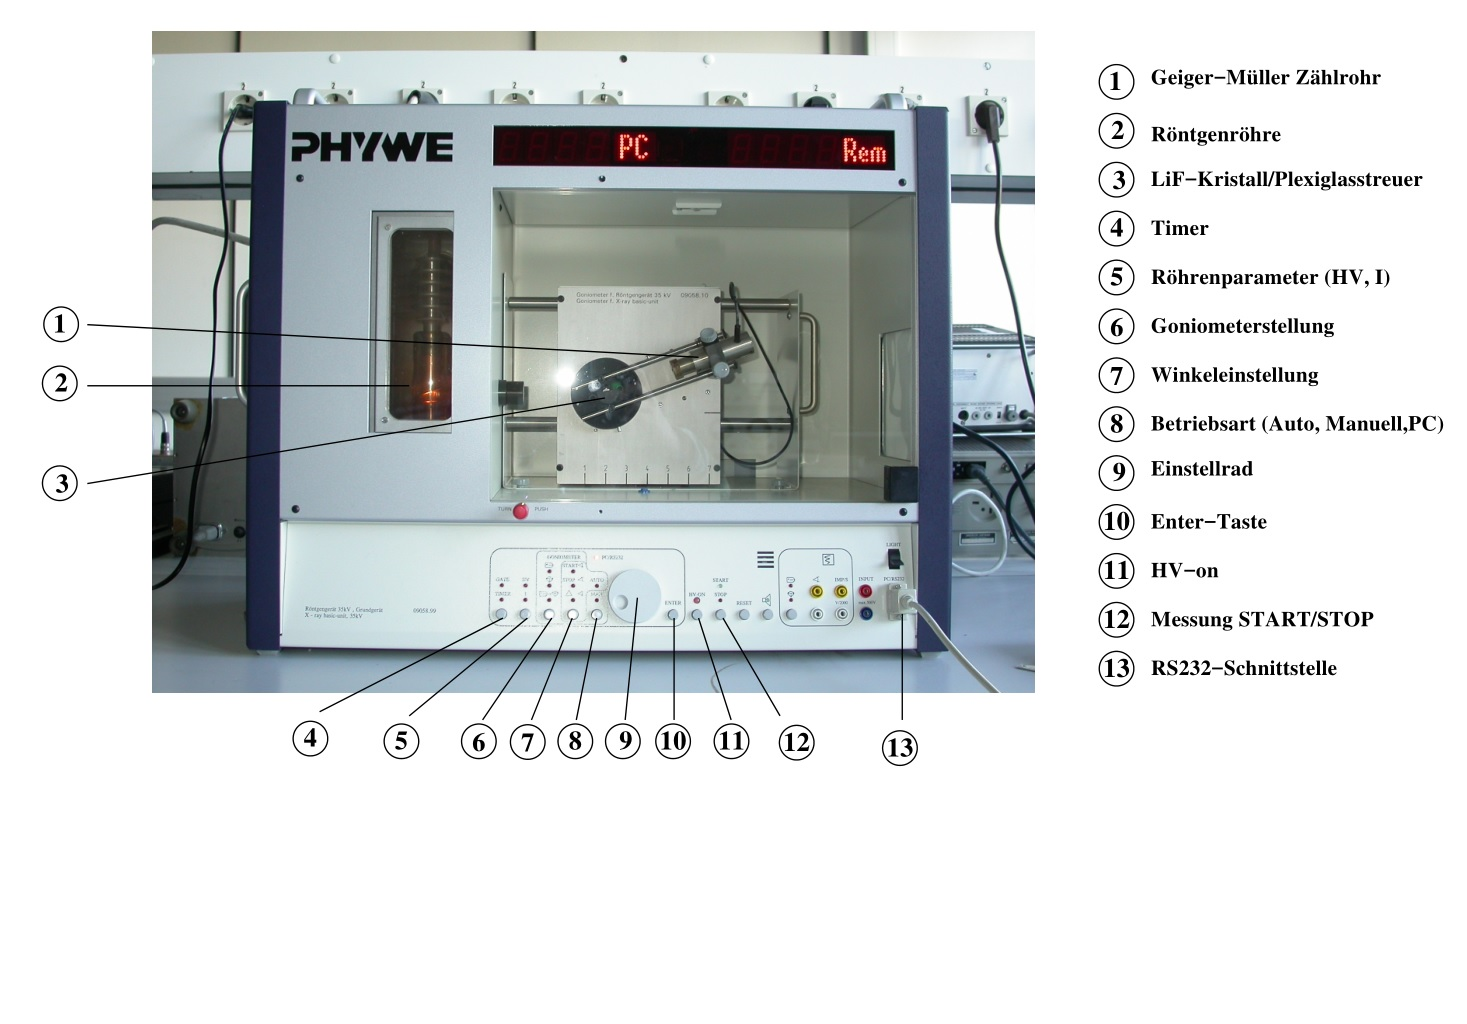
\includegraphics[width=\textwidth]{content/data/aufbau.jpg}
    \caption{Aufbau eines Röntgengeräts. \cite[3]{anleitung}}
    \label{fig:aufbau}
\end{figure}
Die Röntgenröhre soll eine Beschleunigungsspannung von $\SI{35}{\kilo\volt}$ und einen Emissionsstrom von $\SI{1}{\milli\ampere}$ erhalten.
Um das Emissionsspektrum und die Transmissionskurve zu messen wird der LiF-Kristall in die vorgesehene Halterung gesteckt.
\begin{figure}
    \centering
    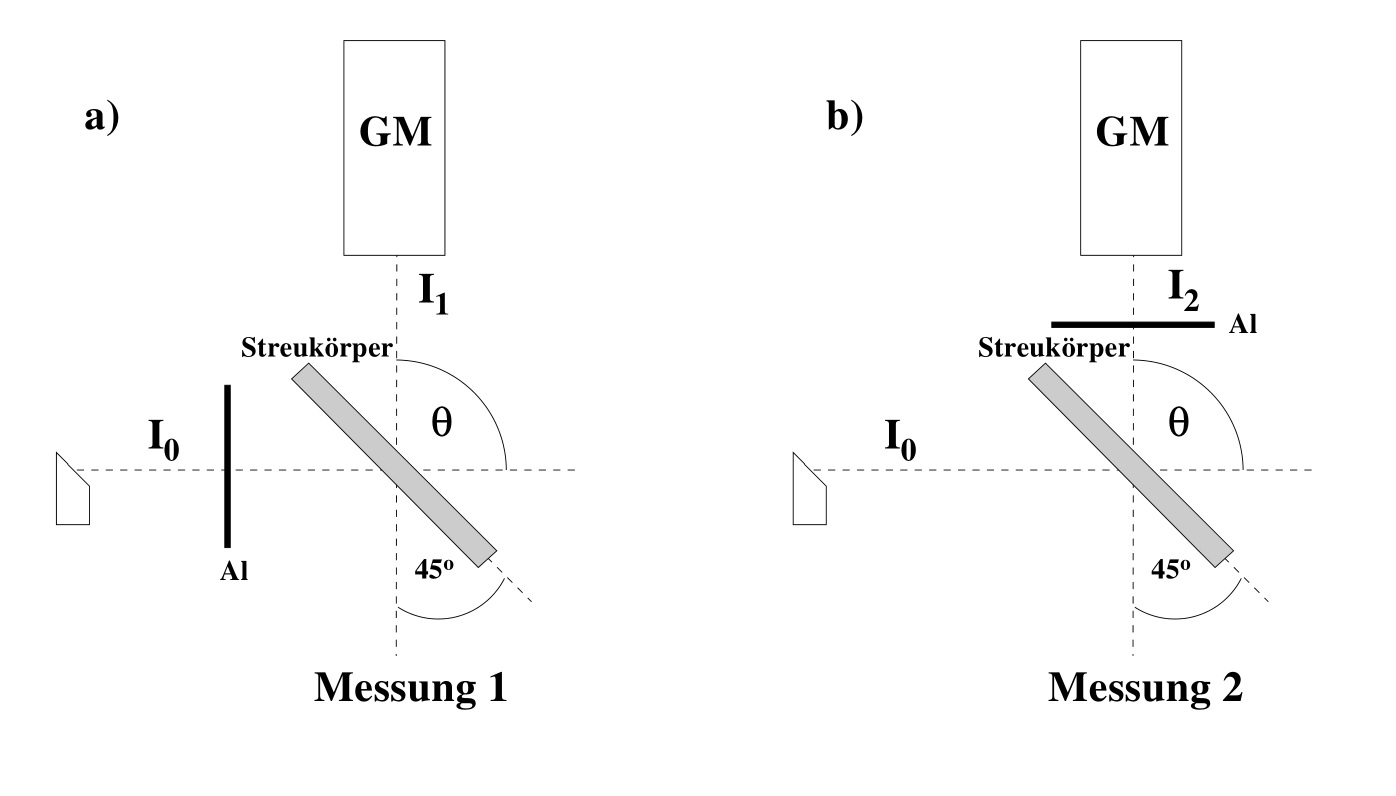
\includegraphics[width=0.5\textwidth]{content/data/aufbau2.jpg}
    \caption{Experimenteller Aufbau graphisch veranschaulicht. \cite[4]{anleitung}}
    \label{fig:aufbau2}
\end{figure}
%Aufgabe 1
Zuerst soll das Emissionsspektrum mithilfe des Computers gemessen werden.
Dazu wird eine $\SI{2}{\milli\metre}$ Blende und der LiF-Kristall benötigt.
Nun wird das Röntgenspektrum von $\SI{8}{\degree}$ bis $\SI{25}{\degree}$ in $\SI{0.1}{\degree}$-Schritten gemessen.
Die Messzeit pro Winkel beträgt $\SI{10}{\second}$.
\\
%Aufgabe 2
%a)
Im Anschluss wird der Aluminium-Absorber vor die $\SI{2}{\milli\metre}$ Blende gesetzt und $N_\text{Al}$ bei einer Messzeit von $t=\SI{100}{\second}$ gemessen.
Bei der selben Messzeit wird $N_0$ ohne Absorber gemessen.
Die Zählrate muss von $\SI{7}{\degree}$ bis $\SI{10}{\degree}$ nach
\begin{equation}
    I = \frac{N}{1 - \tau \cdot N}
    \label{eqn:totzeit}
\end{equation}
korrigiert werden.
Das Geiger-Müller-Zählrohr hat eine Totzeit von $\SI{90}{\micro\second}$.
Aus der Zählrate folgt die Transmission $T(\lambda) = \frac{I_\text{Al}}{I_0}$.

%b)
Nun wir die $\SI{2}{\milli\metre}$ Blende durch eine $\SI{5}{\milli\metre}$ Blende ersetzt und der LiF-Kristall durch einen Plexiglas-Streuer ausgetauscht.
Der Kristall wird auf $\SI{45}{\degree}$ und das Geiger-Müller-Zählrohr auf $\SI{90}{\degree}$ eingestellt (siehe Abb. \ref{fig:aufbau2}) und im Anschluss die Intensität $I_0$ der Cu-Röhre manuell gemessen.

%c)
Die Messzeit beträgt bei der folgenden Messung $t=\SI{300}{\second}$.
Zuerst soll die Transmission $T_1=\frac{I_1}{I_0}$ für die noch nicht gestreute Röntgenstrahlung gemessen werden.
Dazu wird der Aluminiumabsorber in den Strahlengang zwischen Röntgengerät und Streukörper gebracht (siehe Abb. \ref{fig:aufbau2}).
Danach wird der Aluminiumabsorber in den Strahlengang zwischen Streukörper und Geiger-Müller-Zählrohr gebracht (siehe Abb. \ref{fig:aufbau2}) und die Transmission $T_2=\frac{I_2}{I_0}$ für die gestreute Röntgenstrahlung bestimmt.